
\begin{tehtava}
\item\( F = ma\,; \quad m = \text{?}\)\item\( A = \pi r^2\,; \quad r = \text{?}\)\item\( a_n = \frac{v^2}{r}\,; \quad v = \text{?}\)\item\( v = v_0 + at\,; \quad a = \text{?}\)\end{kohdat}
\end{tehtava}

\begin{tehtava}
Ratkaise yhtälöistä \(x\).
\begin{kohdat}
\item \(ax = 2x + 1\)
\item \(2t\sqrt{x} = 3\e^t - t\)
\end{kohdat}
\end{tehtava}

\begin{tehtava}
Ratkaise yhtälö
\begin{kohdat}
\item \( x(\sqrt{2} - 1) = 1 - 2x \)
\item \( (1-x)^2 + 3(2x+1) = (2+x)^2 \)
\end{kohdat}
\end{tehtava}

\begin{tehtava}
Ratkaise yhtälö
\begin{kohdat}
\item \( 5x + 7 = 8x + 4 \)
\item \( 3x - 5(2x - 6) = 0 \)
\item \(\displaystyle \frac{x}{4} - \frac{2x-1}{3} = \frac{5}{6}\)
\end{kohdat}
\end{tehtava}

\begin{tehtava}
Ratkaise yhtälö
\begin{kohdat}
\item \((x + 2)(3x - 4) = 0\)
\item \(5x^2 - 2x = 0\)
\item \(4x^2 - 3 = 0\)
\item \(9x^2 + 1 = 0.\)
\end{kohdat}
\end{tehtava}

\begin{tehtava}
Ratkaise yhtälö.
\begin{kohdat}
\item \(2x^2 - 5x + 3 = 0\)
\item \((x - 5)(1 - 3x) = 7\)
\item \(3x^2 - x = -1\)
\end{kohdat}
\end{tehtava}

\begin{tehtava}
Olkoon $f(x)=x^2$. Laske
\begin{kohdat}
\item \(f(2)\)
\item \(f(-5).\)
\end{kohdat}
\end{tehtava}

\begin{tehtava}
Olkoon $$f(x)=\frac{2^x+4}{x}.$$ Laske, mikäli mahdollista:
\begin{kohdat}
\item \(f(2)\)
\item \(\displaystyle f\left(\frac{1}{3}\right)\)
\item \(f(0)\)
\item \(f(-1)\)
\end{kohdat}
\end{tehtava}

\begin{tehtava}
Missä kohdassa funktiot $ g(x)=5^{x} $ ja $\displaystyle h(x)=\left(\frac{1}{4}\right)^{x} $ saavat saman arvon?
\end{tehtava}

\begin{tehtava}
Luvun $x$ itseisarvo $|x|$ määritellään seuraavasti:\[|x| =\begin{cases}x, & \text{ jos $x\ge 0$} \\-x, & \text{ jos $x < 0$}.\end{cases}\]Piirrä funktion $f(x)=|x|$ kuvaaja.
\end{tehtava}

\begin{tehtava}
Piirrä funktion \(f\colon\R\to\R\), $f(x)= 5$ kuvaaja.
\end{tehtava}

\begin{tehtava}
Määritellään funktio $f$ seuraavasti:\[f(x) =\begin{cases}0, & \text{ jos } x < 0 \\x+1, & \text{ jos } x \geq 0.\end{cases}\]Piirrä funktion $f$ kuvaaja.
\end{tehtava}

\begin{tehtava}
Mitä funktiota seuraava kuvaaja esittää?\begin{center}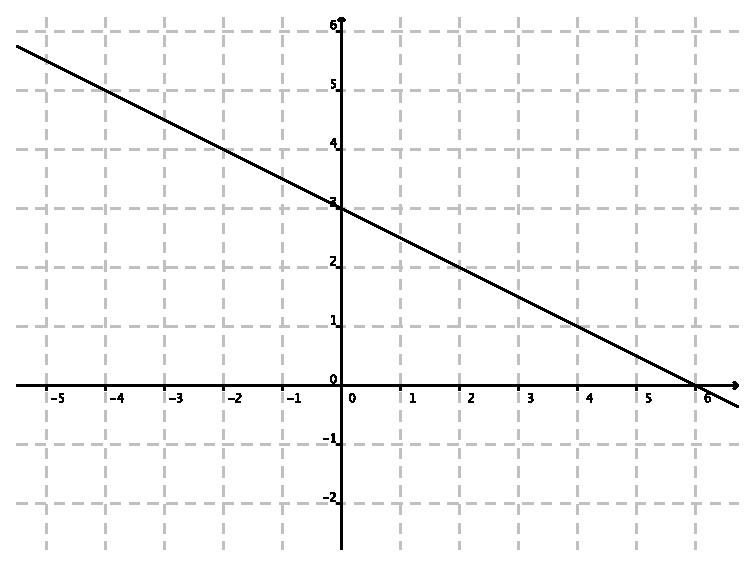
\includegraphics{figs/kuvaaja.eps}\end{center}
\end{tehtava}

\begin{tehtava}
Olkoon $f(x) = (x+5)^3$. Laske
\begin{kohdat}
\item \(f(-2)\)
\item \(f(x-5).\)
\end{kohdat}
\end{tehtava}

\begin{tehtava}
Olkoon neliön sivun pituus $x$. Mikä funktio kuvaa neliön pinta-alaa? Jos kyseessä on kuution pohjaneliö, niin mikä funktio kuvaa kuution tilavuutta? Entä vaipan pinta-alaa?
\end{tehtava}

\begin{tehtava}
Olkoon $f(x)=\sqrt{x}$. Mikä on funktion $f$ arvo pisteessä $32$? Mikä on kuvassa näkyvän funktion arvo pisteessä $4$?\begin{center}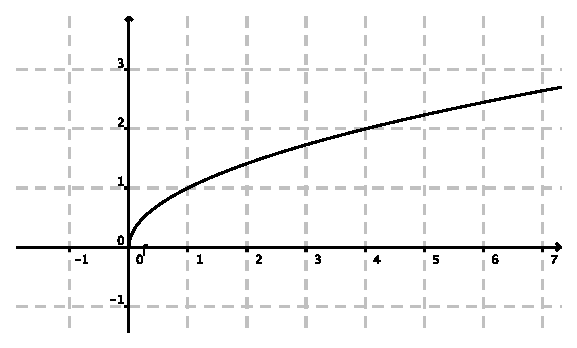
\includegraphics{figs/neliojuuri.eps}\end{center}
\end{tehtava}

\begin{tehtava}
Selvitä funktion $f(x) = x^2 - 4$ nollakohdat. (Toisin sanoen ne luvut $x$, joilla pätee $f(x)=0$.)
\end{tehtava}

\begin{tehtava}
Olkoon $f(x)=2x+9$ ja $g(x)=12x-1$. Millä $x$:n arvolla pätee $f(x)=g(x)$?
\end{tehtava}

\begin{tehtava}
Piirrä funktion $f(x) = 2x-5$ kuvaaja.
\end{tehtava}

\begin{tehtava}
Olkoon $f(x)=-4x^{-3}$ ja $ \displaystyle g(x)=\frac{1}{2}(-x)^{2}$. Määritä
\begin{kohdat}
\item \(f(2)\)
\item \(f(0)\)
\item \(g(-4)\)
\item \(\displaystyle f\left(\frac{1}{2}\right)\cdot g\left(\frac{1}{2}\right)\)
\item \(\displaystyle f\left(g(2)\right).\)
\end{kohdat}
\end{tehtava}

\begin{tehtava}
Hahmottele funktion $h(x) = x^2 -4$ kuvaaja.
\end{tehtava}

\begin{tehtava}
Mitkä seuraavista kuvaajista esittävät funktiota? Kielteisessä tapauksessa perustele, miksei kuvaaja esitä funktiota.\begin{center}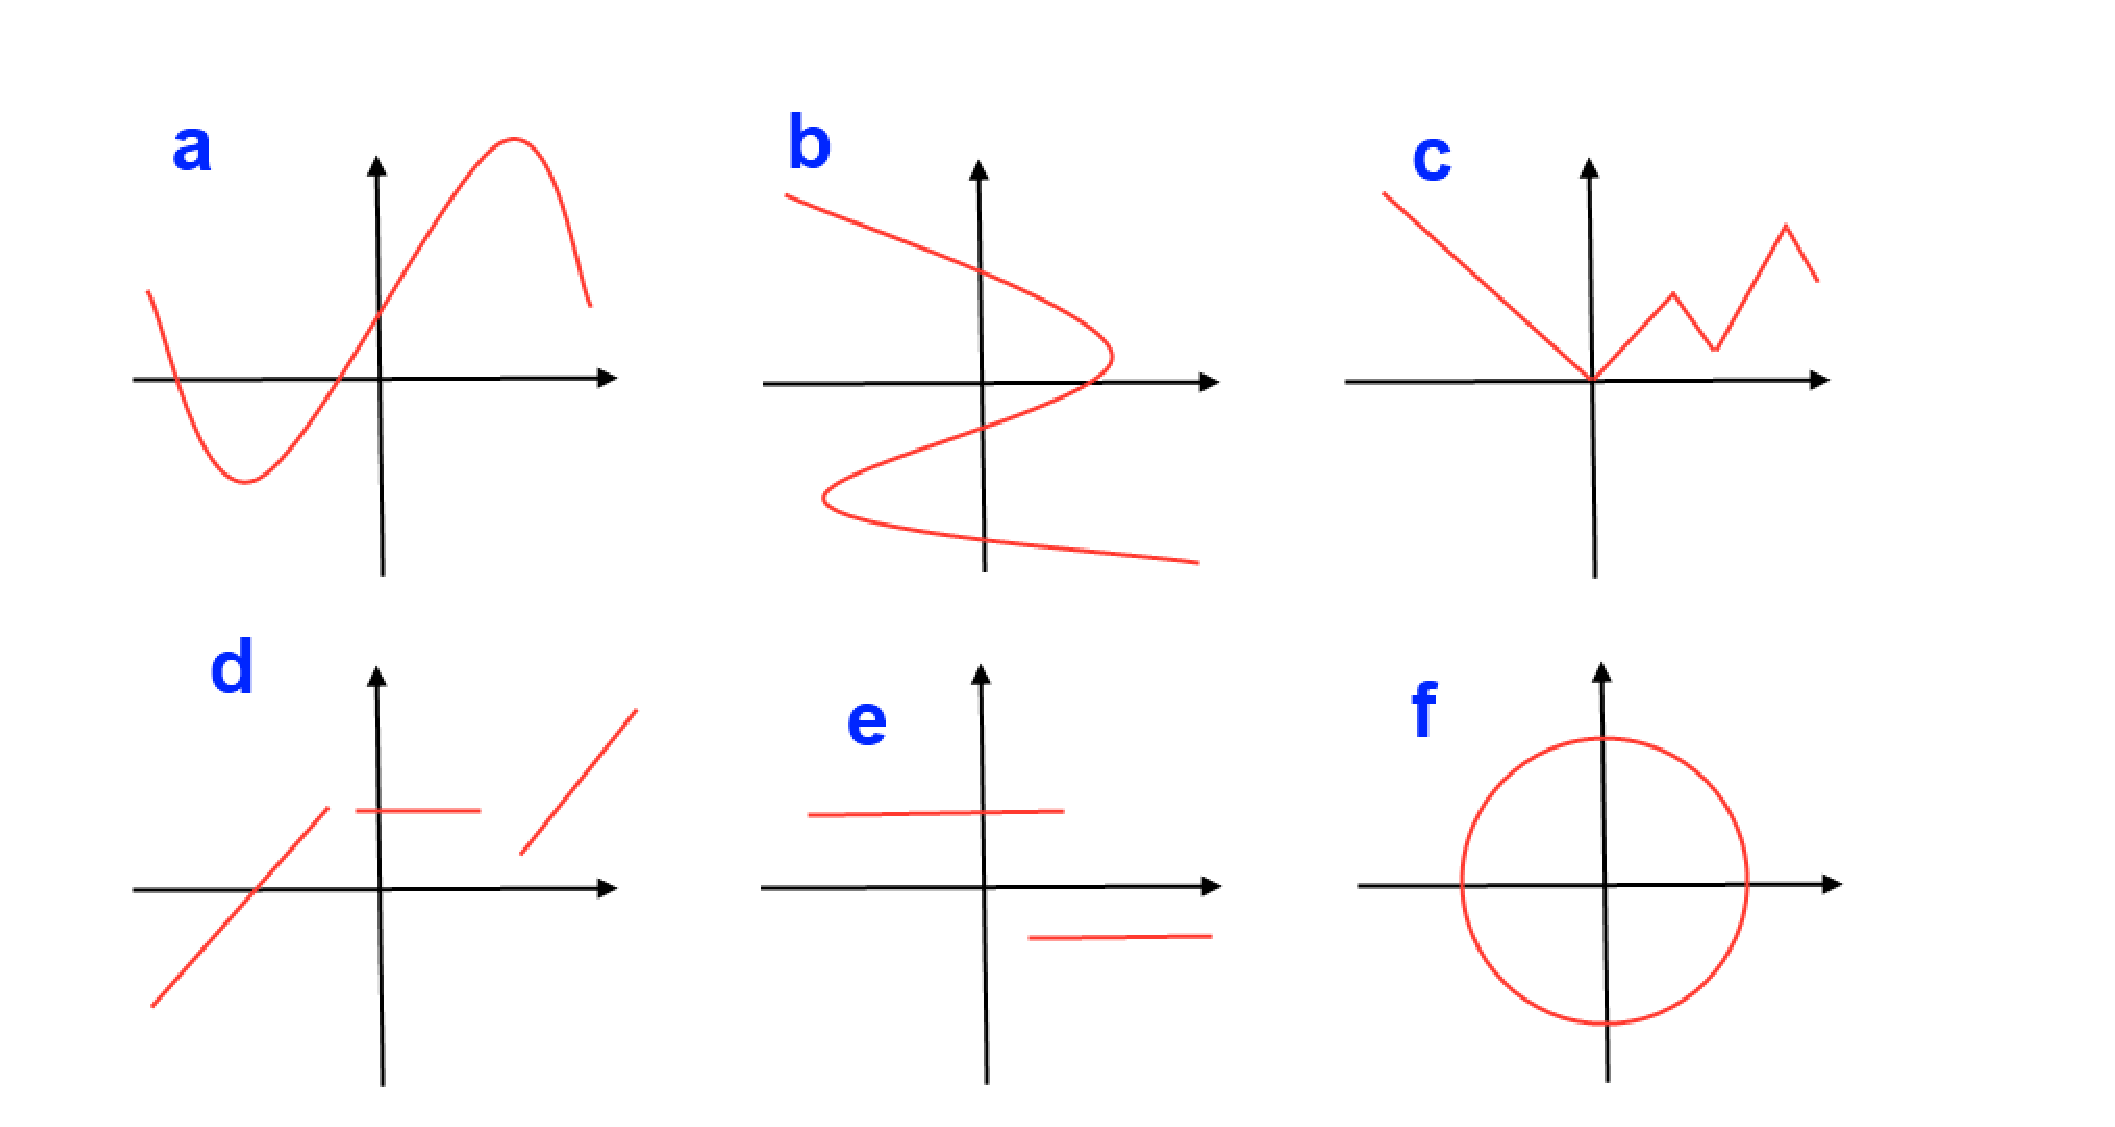
\includegraphics{figs/kuvaajia.eps}\end{center}
\end{tehtava}

\begin{tehtava}
Määritellään funktio $p$ siten, että $p(x)=x+9$, jos $x<5$, ja $p(x) = x/2$, jos $x\ge 5$.Määritä
\begin{kohdat}
\item \( p(6) \)
\item \( p(p(6)) \)
\item \( p(p(p(6)))\)
\end{kohdat}
\end{tehtava}

\begin{tehtava}
Olkoon $f(x) = 2x +1$. Etsi funktio $g$, jolle pätee $g(f(x)) = x$.
\end{tehtava}

\begin{tehtava}
Olkoon $\displaystyle g(x) = \frac{2x-1}{x+1}$. Laske
\begin{kohdat}
\item \(g(2)\)
\item \(g(a-1)\)
\end{kohdat}
\end{tehtava}
